\documentclass[a4paper]{article}

\usepackage{fancyhdr}
\usepackage{parskip}
\usepackage{setspace}
\usepackage[hidelinks]{hyperref}
\usepackage{graphicx} 
\usepackage[margin=1.2in]{geometry}
\graphicspath{ {images/} }
\usepackage[
    backend=biber,
    style=authoryear-icomp,
    sortlocale=de_DE,
    natbib=true,
    url=false, 
    doi=true,
    eprint=false
]{biblatex}
\addbibresource{reference.bib}


\begin{document}

\begin{titlepage}
		
	\center
	
\includegraphics[scale=1]{logo}
	\newcommand{\HRule}{\rule{\linewidth}{0.5mm}}
		
	\textsc{\huge COP531}\\[0.5cm] 
 	\textsc{\huge Wireless Networks}\\[0.5cm]
 
	\HRule\\[0.4cm]

 	{\huge System Design Report}\\[0.4cm]

	\HRule\\[1.5cm]
	\huge\textit{Authors:}
	\begin{minipage}{0.4\textwidth}
 	\begin{center}
   		\large 
   		\textsc{Ameer Ghaffori}
   		\vfill
   		\textsc{Ekow Mensah}
   		\vfill
   		\textsc{Huang Yiwen}
   		\vfill
   		\textsc{Rihui Wang}
   		\vfill
   		\textsc{Zheng Ziheng}
 	\end{center}
 	\end{minipage}

	\vfill\vfill
	{\large\today}
	
\end{titlepage}
	
\newpage
	
\tableofcontents{}
	
\newpage 
	
\section{Problem Definition}
\onehalfspacing 
Technology has become one of the most important aspects of human life. The need for technology and implementation of new technologies and innovations increases daily and annually. The Internet and networking some of the most vital aspects of technology which directly affect various areas of human activities such as work, education, entertainment etc (Yang,2014). Wireless networks are an advanced and modern technology that been found as an alternative to wired technology which uses cables and wires to connect digital devices. A lot of technologies been found and developed in order to support the wireless network technology, such as 3G, 4G, Wifi, Bluetooth, and Zigbee. 


\subsection{Background}	
Wireless sensor networks (WSNs) can be explained as a collection of actuators and sensors which are responsible for controlling and monitoring the remote environment. Situated at various locations, each sensor within the network collectively transports the  data it senses to the main actuator via the network (Yang, 2014). Sohrabi (2014) explains a mobile ad-hoc wireless network as a type of wireless sensor network in which nodes locate neighbours and establish wireless links in order to facilitate transmission and receipt of data in their own way. Furthermore, the network is self-healing and self-forming as it has the ability to adapt to topological changes (addition and removal of nodes) as well as changes in network traffic. The application of wireless sensor networks can be split into two main categories. These are remote tracking and remote monitoring applications and these categories can be further divided into indoor and outdoor tracking and monitoring. Examples include, tracking the enemy's movement in war, detecting forest fires, tracking animal movement within a zoo, monitoring and sensing chemical levels within a factory environment etc (Yang, 2014). 


\parskip 0.2in 

\subsubsection{Protocol stack for wireless sensor networks}
The protocol stack for wireless sensor networks is similar to that of the Open Systems Interconnection (OSI) model but differs in the fact, it does not implement all seven layers of the OSI protocol stack. Rather, this protocol stack implements five of the seven layers of the OSI protocol stack that is, the application layer, transport layer, network layer, data link layer and physical layer. 5 layers are used because, it is not practical to use seven layers in a real WSN application as it becomes very complex and challenging to implement (Yang, 2014). A block diagram of the WSN protocol stack can be seen below in Figure 1.0. 

\parskip 0.2in 

\begin{figure}[!htb] 
  \centering
  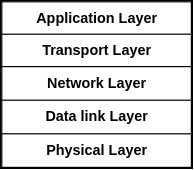
\includegraphics[scale=0.6]{protocolstack}
  \begin{center}
  	\caption{Protocol stack for WSNs}
  \end{center} 
  \label{fig:protocolstack} 
\end{figure}

\subsubsection*{ Physical Layer}
The physical layer handles the definition and management of connections between nodes, additionally, it handles the selection and creation of the carrier frequency, data encryption and frequency modulation (Yang, 2014). Moreover, the physical layer is responsible for the delivery of messages from node to node (Harish \& Sambasivan, 2013).

\subsubsection*{Data Link Layer}
The data link layer ensures the provision of services which enable the access and sharing of a communication medium by several nodes within the network. Examples of these services are media access control (MAC) and error detection and correction (Yang, 2014).
Furthermore, Famry (2016) explains the need for a MAC protocol to handle issues pertaining to data-centric routing and power conservation. The MAC protocol aims to establish a network architecture that is, providing communication links between nodes including self organising abilities and to share communication resources amongst all nodes in the most reasonable and effective manner. A well designed MAC protocol enables channel access in a manner which preserves battery life and improves quality of service.  

\subsubsection*{Network Layer}
The network layer handles the successful routing of packets between nodes including the creation of communication paths between the nodes. The choice of routing protocol controls the manner in which the communication paths are established as each protocol has its own mechanism of determining routes (Yang, 2014). For instance, some routing protocols may decide to select routing paths which will preserve the lifetime of the network whilst others might select routing paths to provide optimum quality of service or if possible, the routing protocol will aim to achieve both (Yang, 2014). The simplest design is to have each node which receives data repeat broadcasts to every neighbour until the destination node receives the data or the maximum hop lifetime has been attained. This approach is known as flooding (Famry, 2016). Although flooding is advantageous in that it is simple and does not require the maintenance of the topology, it is wasteful as it does not consider efficient energy use and causes overlaps between nodes. An relatively better approach to flooding is gossiping. With gossiping, a node arbitrarily chooses a neighbouring node to transmit data to when it receives the data. In spite of the fact that gossiping does solve problem of implosion (i.e. duplicated data being transmitted to the same node), it causes transmission delays (Famry, 2016). Other alternatives that can be used are flat routing protocols such as the Sensor Protocol for Information via Negotiation (SPIN), Direct Diffusion (DD), hierarchical routing protocols such as Low-Energy Adaptive Clustering Hierarchy (LEACH), location based routing protocols such as Geographic Adaptive Fidelity (GAF) and many more. A routing protocol is selected based on the nature of the application of the wireless sensor network.

\subsubsection*{Transport Layer}
The transport layer oversees steadfast communication between end points. While various transport layer protocols exist, Transmission Control Protocol (TCP) and User Datagram Protocol(UDP) are the most widely used protocols on the transport layer. Transmission control protocol provides reliable data transfer and other services which include congestion control, flow control and error detection (Yang, 2014). Unlike TCP, UDP does not provide reliable data transfer or congestion control, moreover, it does not keep track of connections or the order in which packets arrive.  

\subsubsection*{Application Layer} 
The application layer is the first layer of the protocol stack. The application layer handles encryption and processing of the data that was sensed. It is also responsible for the controlling the manner in which data is stored (Yang, 2014). Additionally, before data is transmitted down the protocol stack, the application layer checks each layer to find out whether each layer possesses the requisite resources required to perform the user's request (Yang, 2014). 

\subsection{The Task}
This report explains the design of a wireless mobile ad-hoc network which makes use of a simplified version of the ad-hoc distance vector routing protocol (AODV). The network was comprised of four nodes that is, a source node, two intermediate nodes and a destination node. The source node contained both a temperature and voltage sensor and was responsible for transmitting data (temperature $^\circ$C and battery level $V$) to the destination node, while the intermediate nodes were responsible for relaying packets between the source and destination nodes. The destination node being the coordinator was connected to a dedicated computer and was responsible for displaying the information sent from the source node. The temperature and voltage readings obtained by the source node was transmitted to the destination node every two seconds via the intermediate nodes. The source node selected the next hop node during transmission of the data based on the battery level and radio signal strength indicator (RSSSI) by analysing the information received by the intermediate nodes. This was done in order to make the ad-hoc network more resilient and long lasting. This will be explained in more detail in the system design section.
\newpage

\section{System Design}

This section discuses the design of the mobile ad-hoc wireless network(MANET) including the routing algorithm and a flowchart of the system to be implemented. 



\subsection{Our protocol stack}
In this system, a simple wireless sensor network consisting of four sensor nodes is designed and implemented using the Contiki Operation System. That is, a sender node S, two router nodes T1 and T2, and one receiver node R as shown in figure 2.

\begin{figure}[!htb] 
  \centering
  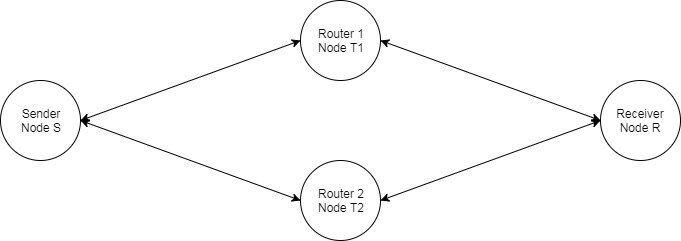
\includegraphics[scale=0.6]{protocolstack2}
  \begin{center}
  	\caption{A 4 nodes WNS}
  \end{center} 
  \label{fig:protostack2} 
\end{figure}

When the node S is to send a data to the destination node R for the first time, there is no available route in the routing table. Then the source node S broadcasts a router request packet (RREQ) across the network and every node within the communication range can receive the request. If an intermediate node receives a RREQ packet, it sets up a reverse route toward to the node where the RREQ packet

is received from. Then, the current intermediate node increases the hop count and rebroadcasts RREQ if it has no route to the destination node. Until the RREQ is received by the destination node, the node sends back a route reply packet (RREP) by following the reverse route. When the intermediate node receives the RREP, it sets up a forward table including the next hop to the destination and re-unicast the RREP to the source node. An available route is being built when the source node receives the RREP and then the data packet can be sent according to the forward table in each node. This is the route discovery mechanism to find any possible paths from the source device to the destination device.  

\subsection{Routing Principle}
When a route discovery is required, the sender broadcasts RREQ and waits for the responding from the destination. A routing algorithm need to be designed to figure out the best path if the available routes are more than once. In this system, the battery level and received signal strength indication (RSSI) of the intermediate node will be gathered and send to the source device. The source device compares the battery level with the average level. Then the source node compares the RSSI if the battery level of the intermediate nodes is higher than the average level and choose the route with higher signal strength. If the battery level of the intermediate nodes is lower than the average level, the source node will select the route with higher battery level. The whole process to figure out the best route is shown in figure 3.

\begin{figure}[!htb] 
  \centering
  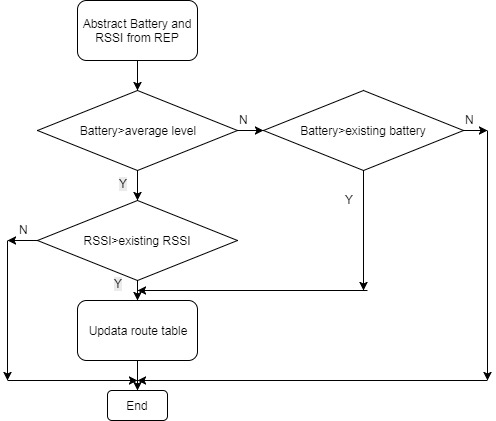
\includegraphics[scale=0.6]{routingdiagram}
  \begin{center}
  	\caption{The process to find the best path (Yang, 2014)}
  \end{center} 
  \label{fig:protocolstack2} 
\end{figure}


For the RREQ, a broadcast count is included to guarantee the data packet sent by the source device takes two or more hops to the destination. The destination node only processes the RREQ with the number of count higher than 1. Meanwhile, the broadcast will be deleted if the number of count is higher than 3 to avoid implosion.

There may be circumstances that the signal strength from the intermediate nodes changes. Therefore, the routing table should be updated in real time, which means the sender node keeps sending RREQ messages all the time to guarantee the best path is always stored in the routing tables.

There may be circumstances that the intermediate node runs out of battery, but the sender still sends data packet to this intermediate node since the routing table is not updated. Therefore, a data identification number is created in the data packet and transmitted along with the data. When the destination node receives the data packet, it identifies the data identification number and sends it back to the source node along with the RREP messages. The routing table will be reset if the source node finds that the identification number received from the destination node is smaller than the current identification number by three, which means the lost data packets are more than three.


\subsection{Embedded Software Design (Flowcharts)}

There are three types of nodes in this system: sender, router and receiver. For the sender, it is capable of sending data packet or RREQ, and receiving the RREP through unicast from the intermediate nodes.
To be more detail, in this system, the sender broadcasts the RREQ every two seconds to all its neighbours within the communication range. When the sender receives the unicast of RREP from the router, it updates the routing table according to battery level and RSSI of the intermediate node to guarantee the routing table always keeps the best path. Then the sender unicasts the data packet every two seconds to the next hop stored in the routing table. The flow chart for the sender is shown in figure 4.

\begin{figure}[!htb]
   \centering
   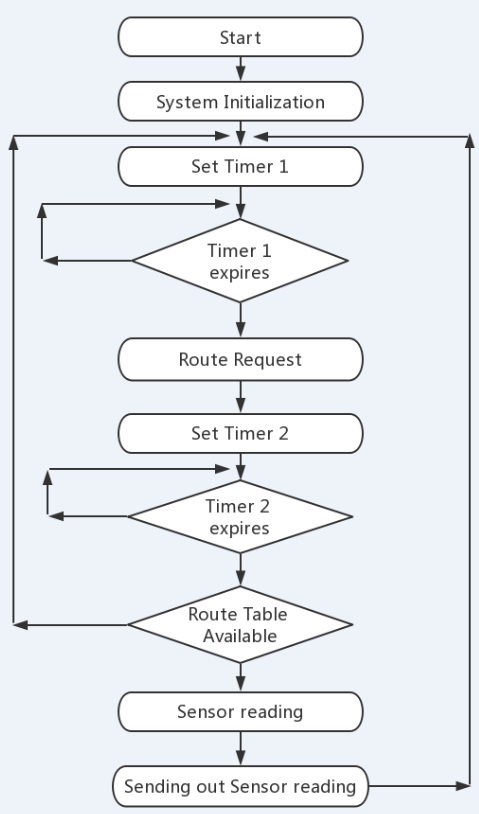
\includegraphics[scale=0.4]{flowchart1}
	\begin{center}
	   \caption{Flowchart of the sender (Yang, 2014)}
	\end{center}	   
    \label{fig:flowchart1}
\end{figure}

For the router, it rebroadcasts the RREQ if the count number is lower than three when it receives the RREQ from the source node. If a unicast message is received, then it retransmits the RREP packet or the data packet to the source node and destination respectively. The flow chart for the router is shown in figure 5.

\begin{figure}[!htb]
   \centering
   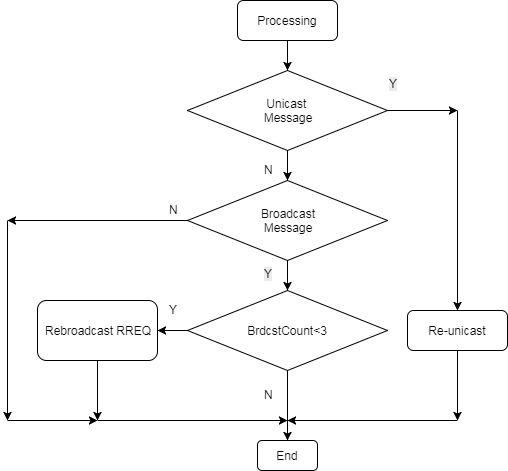
\includegraphics[scale=0.6]{flowchart2}
	\begin{center}
	   \caption{The flowchart of the router}
	\end{center}	   
    \label{fig:flowchart2}
\end{figure}


For the receiver, print out the data message when it receives a unicast from the intermediate node and send back a RREP when it receives the broadcast. The flow chart of the receiver is shown in figure 6.

\begin{figure}[!htb]
   \centering
   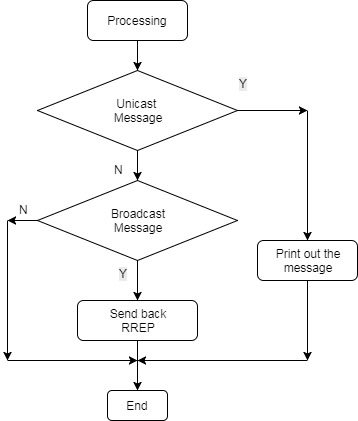
\includegraphics[scale=0.5]{flowchart3}
	\begin{center}
	   \caption{The flowchart of the receiver}
	\end{center}	   
    \label{fig:flowchart3}
\end{figure}

\subsubsection*{The type of messages: (Yang, 2014)} 
Route Request Message:\\
Type (8 bit): identifies the type of message (COMMAND\_ROUTEREQUEST)\\
Destination address (16 bit):  the Rime address of the destination for which a route is required \\
Broadcast counter (8 bit): specifies how many times the current message has been sent \\
Broadcast limit (8 bit): the maximum number of times a message can sent by broadcast \\
Broadcast id (8 bit): identification number of the current broadcast message \\

Route Reply Message: \\
Type (8 bit): identifies the type of message (COMMAND\_ROUTERESPONSE)\\
Destination address (16 bit):  the Rime address of the destination for which a route is given \\
Battery (16 bit): the battery level of the destination node \\
Nomessage (8 bit): the identification of the data id received in the receiver \\

Data Transmission Message:\\
Type (8 bit): identifies the type of message (COMMAND\_DATATX) \\
Destination address (16 bit):  the Rime address of the destination of the sensed data \\
Source address (16 bit):  the Rime address of the source of the transmitted data \\
Temperature (16 bit): the sensed temperature data to be transmitted \\
Battery (16 bit): the battery level data to be transmitted \\
Data id (8 bit): identification number of the current broadcast message \\

Reverse table: \\
BrdcstID: to identify the broadcast message (8 bit) \\
From: the source device from which the route request is obtained (16 bit) \\
Dest: the address of the destination for which a route is required (16 bit) \\

Routing Table: \\
Dest: the address of the destination (16 bit) \\
NextHop: The next hop required to reach the destination (16 bit)  \\
Battery: Battery level of the nodes (16 bit) \\
RSSI: The received signal strength indication (16 bit) \\

\section{Test Procedure and Evaluation}

\subsection{Description}

There are mainly two kinds of testing. In the first testing, four sensor nodes are used, one sender, two routers and one receiver respectively. Figure 7 shows the topology of the first test. And this test prove that this wireless system implement the fundamental functions.

\begin{figure}[!htb]
   \centering
   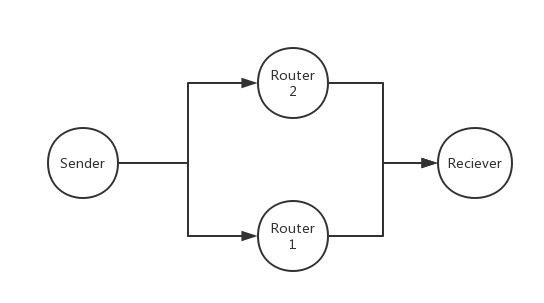
\includegraphics[scale=0.5]{testtopology1}
	\begin{center}
	   \caption{Topology in fundamental test}
	\end{center}	   
    \label{fig:testtopology1}
\end{figure}

Totally, there are three conditions. The first condition is both of router1 and router2 are switched on. The second one is router1 is switched off and router2 is switched on. The last condition is that router2 is switched off and router1 is switched on. In each condition three functions, namely broadcast(RREQ), unicast(RREP) and the send data are tested. 
Except for the fundamental functions test, more sensor nodes are joined to the system to prove that this system implement some extra functions. The figure shows the topology of the extra test. 

\begin{figure}[!htb]
   \centering
   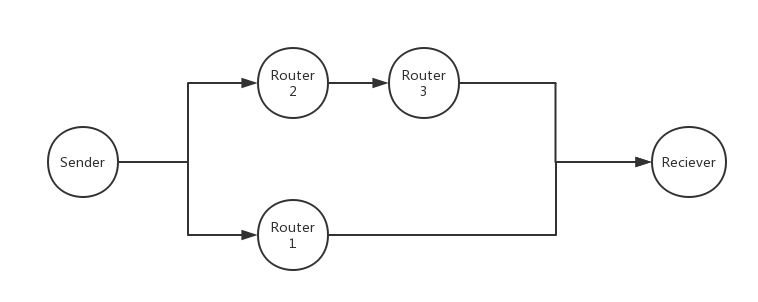
\includegraphics[scale=0.5]{testtopology2}
	\begin{center}
	   \caption{Topology in extra test}
	\end{center}	   
    \label{fig:testtopology2}
\end{figure}

It is clear that there are three routers. There are two conditions to be tested. The first one is that all routers are switched on. The second condition is that the router1 is switched off. Similar to the fundamental test, three functions, broadcast(RREQ), unicast(RREP) and the send data are tested. To make the test easier to understand, all the packet information is displayed by all sensor node including sending packet out and receiving packet and will be shown as screenshots.

\subsection{Fundamental Test}
As shown in the figure 7, there are four sensor nodes. MAC address of all sensor nodes are modified.  It is shown in the table 1.

\begin{table}[!htb]
 \centering
 \begin{tabular}{|c|c|}
 \hline
  Sensor node & MAC address \\
  \hline
  Sender & 00::00:AA:AA \\
  \hline 
  Router1 & 00::00:BB:BB \\
  \hline
  Router2 & 00::00:CC:CC \\
  \hline
  Receiver &00::00:DD:DD \\
  \hline
 \end{tabular}
 \textbf{\caption{Table showing the sensor node and corresponding MAC address}}
\end{table}

\subsubsection{Broadcast Test (RREQ)}

When all sensor nodes are switched on, the broadcast(RREQ) should be sent out by the sender which address is AA:AA. Then the broadcast will be received by two routers and two routers rebroadcast.

\begin{figure}[!htb]
   \centering
   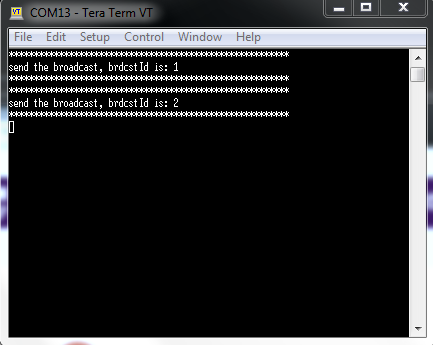
\includegraphics[scale=0.7]{test1}
	\begin{center}
	   \caption{Sender transmits broadcast}
	\end{center}	   
    \label{fig:test1}
\end{figure}

\begin{figure}[!htb]
   \centering
   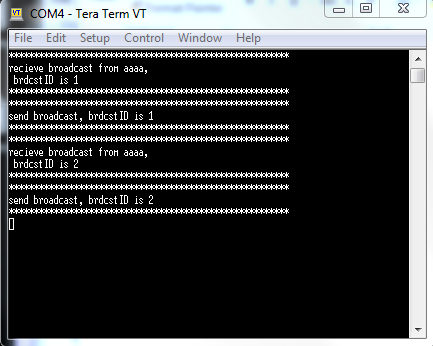
\includegraphics[scale=0.7]{test2}
	\begin{center}
	   \caption{Router received the broadcast}
	\end{center}	   
    \label{fig:test2}
\end{figure}

As the figure 9 shown, two broadcast is sent out and broadcast ID is 1 and 2. In figure 10, it is clear that routers receive the broadcast and the packet is from AA:AA which is the address of sender. When the routers receive the broadcast from sender it need to rebroadcast. And the broadcast ID is unchanged. Therefore, it is proved that the broadcast function is implemented by the sender and routers. What is needed to be explained is the broadcast ID which is used to avoid the broadcast storm. When the routers receive broadcast, it need to rebroadcast to find the next node. Rebroadcast causes that the routers receive the same broadcast from other routers and rebroadcast again. Obviously it will be an infinite loop. To solve this problem. The broadcast ID is used. When the routers receive the broadcast, it will check the broadcast ID firstly. If it is equal to the old one, routers will update the tables but not broadcast it again.
When routers receive the broadcast and rebroadcast. The receiver should receive broadcast. The figure 11 shows that the receiver receives the broadcast from routers.

\begin{figure}[!htb]
   \centering
   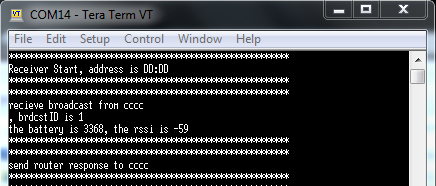
\includegraphics[scale=0.8]{test3}
	\begin{center}
	   \caption{Receiver getting broadcast}
	\end{center}	   
    \label{fig:test3}
\end{figure}

There is a problem that the receiver only can receive one broadcast from router2(CC:CC). The reason is that the router2 is closer to the receiver and the receiver get the broadcast from router2 first. And the receiver will handle the broadcast which causes receiver cannot receiver other broadcast like the broadcast from router1(BB:BB).

\subsubsection{Unicast(RREP) test}

When the receiver get the unicast, it should be able to solve the broadcast and choose a better router according to hop counts battery and RSSI. In this case the hop counts are the same in the two path. Therefore only battery and RSSI need to be considered.

\begin{figure}[!htb]
   \centering
   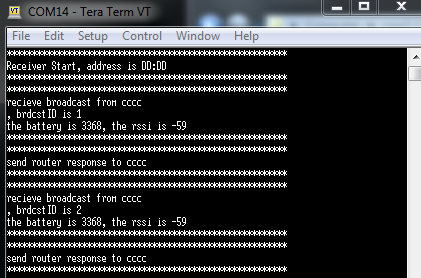
\includegraphics[scale=0.8]{test4}
	\begin{center}
	   \caption{Unicast to router}
	\end{center}	   
    \label{fig:test4}
\end{figure}

From figure 12 it is clear that the receiver chooses the router2(CC:CC) and send unicast to it. What is needed to be declared is that the hop-counts has the best priority. Battery has the second priority and the RSSI is the last. In this case the hop-counts are the same and the battery need to be compared. The router2 has higher battery so it is chosen.
After that the router2 need to receive the unicast and send another unicast to the sender.

\begin{figure}[!htb]
   \centering
   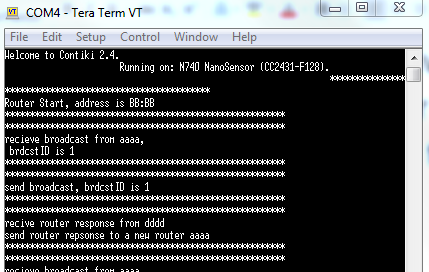
\includegraphics[scale=0.8]{test5}
	\begin{center}
	   \caption{Unicast to router}
	\end{center}	   
    \label{fig:test5}
\end{figure}

From figure 13 it is clear that the router2 receive the RREP from the router (DD:DD) and send it to the last hop which is the receiver (AA:AA). After the router send the RREP to the sender, the path from sender and receiver is established which means the routing process is finished.

\subsubsection{Data transfer test}

After the path is established, it is supposed that the sender can send to the router using the path. In this test, sender sent data packet continuously to the receiver by push the button2. 

\begin{figure}[!htb]
   \centering
   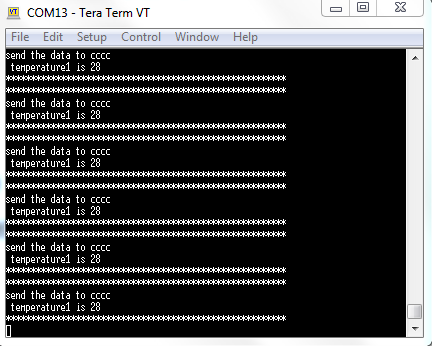
\includegraphics[scale=0.8]{test6}
	\begin{center}
	   \caption{Data packet from sender}
	\end{center}	   
    \label{fig:test6}
\end{figure}

\newpage
From figure 14 it is clear that the data is sent to router2(CC:CC) first. Because it was chosen in the routing process.


\begin{figure}[!htb]
   \centering
   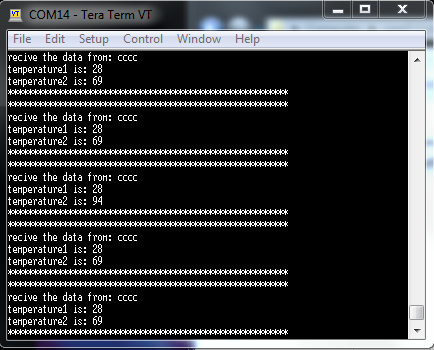
\includegraphics[scale=0.8]{test7}
	\begin{center}
	   \caption{Receiver receives data}
	\end{center}	   
    \label{fig:test7}
\end{figure}


From figure 15, it is clear that the content of the data is the same as what is sent out from the sender. In this test, only the temperature is chosen as the testing feature. And the data is from the router2(CC:CC). It proves that there is only one path in the topology which means the path is established successfully.

\subsection{Extra Tests}

In the extra test, there are five routers in the topology. From figure 8, it can be seen that there are three routers, one receiver and one sender. In this part, two conditions will be tested. The first one is all router are switched on and second one is that the router1 is switched off. This test aims to prove that router can choose shorter path and when the path is broken it can establish new path. Details in the test will not be discussed and some main parts will be introduced. Address of each sensor node is displayed in the table2.

\begin{table}[!htb]
 \centering
 \begin{tabular}{|c|c|}
 \hline
  Sensor node & MAC address \\
  \hline
  Sender & 00::00:AA:AA \\
  \hline 
  Router1 & 00::00:BB:BB \\
  \hline
  Router2 & 00::00:CC:CC \\
  \hline
  Router3 & 00::00:FF:FF \\
  \hline
  Receiver &00::00:DD:DD \\
  \hline
 \end{tabular}
 \textbf{\caption{Address of each sensor node in the test}}
\end{table}

\subsubsection{All Routers Switched On}

In this test, when the path is established, the sender need to send data to router1 first.

\begin{figure}[!htb]
   \centering
   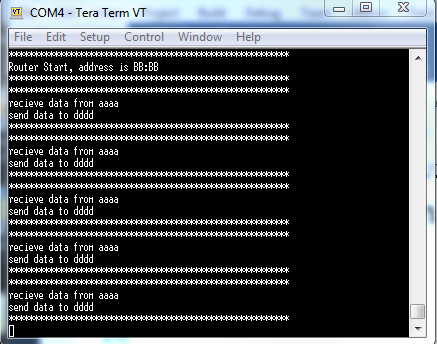
\includegraphics[scale=0.8]{test8}
	\begin{center}
	   \caption{router1 receive the data}
	\end{center}	   
    \label{fig:test8}
\end{figure}

\subsubsection{Router1 switched off}

If the router1 is switched off, when sender send data to receiver, it need to use router2 and router3. So router 2 and router3 are all supposed to receive the data and finally the receiver receive data from router3. The topology is as shown in figure 17.

\begin{figure}[!htb]
   \centering
   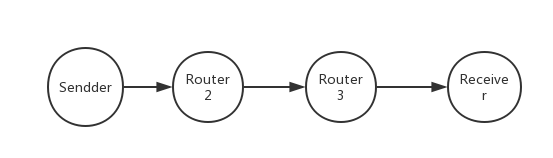
\includegraphics[scale=0.8]{chart4}
	\begin{center}
	   \caption{Topology of two routers in one path}
	\end{center}	   
    \label{fig:chart4}
\end{figure}

\begin{figure}[!htb]
   \centering
   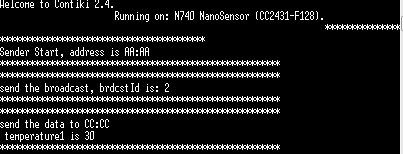
\includegraphics[scale=0.8]{test9}
	\begin{center}
	   \caption{Sender sent the data}
	\end{center}	   
    \label{fig:test9}
\end{figure}

\begin{figure}[!htb]
   \centering
   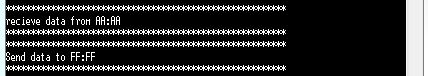
\includegraphics[scale=0.8]{test10}
	\begin{center}
	   \caption{Router received the data}
	\end{center}	   
    \label{fig:test10}
\end{figure}

\begin{figure}[!htb]
   \centering
   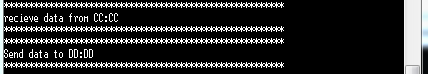
\includegraphics[scale=0.8]{test11}
	\begin{center}
	   \caption{Router receive the data and sent it to another router}
	\end{center}	   
    \label{fig:test11}
\end{figure}

\begin{figure}[!htb]
   \centering
   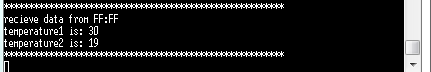
\includegraphics[scale=0.8]{test12}
	\begin{center}
	   \caption{Receiver received the data}
	\end{center}	   
    \label{fig:test12}
\end{figure}

From the images, the sender sends out the data out. And router2 receive the data and transfer it to router3. Finally, router3 send data to receiver.

\newpage
\section{Reference List}


	
\end{document}